\documentclass[border=2pt]{standalone}
\usepackage{tikz}
\usepackage{pgfplots}
\pgfplotsset{compat=1.18}

% Brand colors
\definecolor{Garnet}{rgb}{0.451, 0.0, 0.039}
\definecolor{Atlantic}{rgb}{0.275, 0.416, 0.624}
\definecolor{Congaree}{rgb}{0.122, 0.255, 0.302}
\definecolor{Horseshoe}{rgb}{0.396, 0.471, 0.043}
\definecolor{Rose}{rgb}{0.8, 0.18, 0.251}
\definecolor{Honeycomb}{rgb}{0.643, 0.569, 0.216}
\definecolor{Grass}{rgb}{0.808, 0.827, 0.094}
\definecolor{Black90}{rgb}{0.212, 0.212, 0.212}
\definecolor{Black70}{rgb}{0.361, 0.361, 0.361}
\definecolor{Black50}{rgb}{0.635, 0.635, 0.635}

\begin{document}
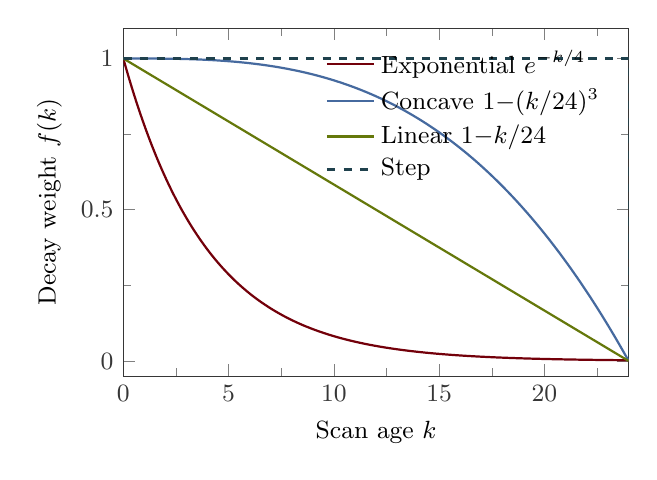
\begin{tikzpicture}
\begin{axis}[
  width=8cm,
  height=6cm,
  xmin=0, xmax=24,
  ymin=-0.05, ymax=1.1,
  xlabel={Scan age $k$},
  ylabel={Decay weight $f(k)$},
  xlabel style={font=\small},
  ylabel style={font=\small},
  xtick align=inside,
  ytick align=inside,
  minor tick num=1,
  axis line style={Black90},
  tick label style={font=\small, color=Black90},
  legend style={
    at={(0.97,0.97)},
    anchor=north east,
    draw=none,
    fill=none,
    font=\small,
    cells={anchor=west}
  },
  axis on top=false,
  enlarge x limits=false,
  enlarge y limits=false,
  rounded corners=0pt,
  every axis plot/.append style={line width=1.2pt}
]

% Exponential: f(k) = exp(-k/4)
\addplot[color=Garnet, solid, thick, domain=0:24, samples=200]
  {exp(-x/4)};
\addlegendentry{Exponential $e^{-k/4}$}

% Concave: f(k) = max(0, 1-(k/24)^(1/3))  --  concave means slower decay then cliff
% Interpreted as a concave-down shape: f(k) = (1 - k/24)^(1/3)
% But user said max(0, 1-(k/24)^3) which is a sigmoid-like concave shape
\addplot[color=Atlantic, solid, thick, domain=0:24, samples=200]
  {max(0, 1-(x/24)^3)};
\addlegendentry{Concave $1{-}(k/24)^{3}$}

% Linear: f(k) = 1 - k/24
\addplot[color=Horseshoe, solid, thick, domain=0:24, samples=200]
  {1 - x/24};
\addlegendentry{Linear $1{-}k/24$}

% Step: horizontal line at 1.0 from 0 to 24, then drops to 0
% Render as two segments
\addplot[color=Congaree, dashed, thick]
  coordinates {(0,1.0) (24,1.0) (24,0.0)};
\addlegendentry{Step}

\end{axis}
\end{tikzpicture}
\end{document}
